\section{Положение неметаллов в Периодической системе. Типичные свойства и степени окисления неметаллов. Основные типы соединений, образуемых неметаллами.}

Неметаллические свойства элементов определяются способностью атомов ''принимать'' электроны, т.е. проявлять при взаимодействии с атомами других элементов окислительные свойства.

Неметаллы в таблице Менделеева находятся справа сверху над диагональю от бериллия к астату (см. рисунок \ref{fig:21.mendel}).

\begin{figure}[H]
	\centering
	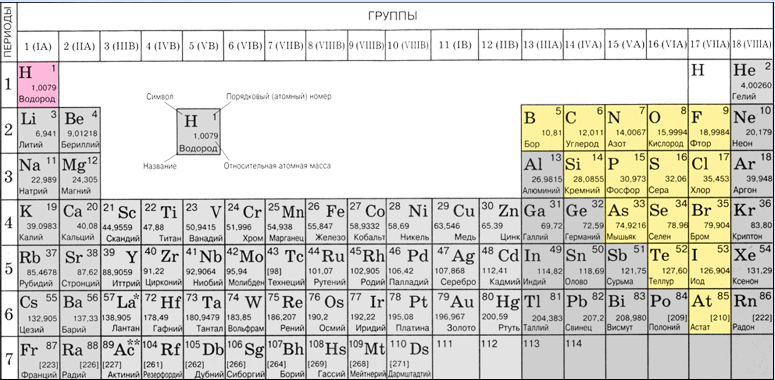
\includegraphics[width=0.7\linewidth]{21.mendel}
	\caption{Положение неметаллов в таблице Менделеева. Выделены цветом.}
	\label{fig:21.mendel}
\end{figure}

Практически все неметаллы имеют сравнительно малые радиусы и большое число электронов на внешнем энергетическом уровне от 4 до 7, для них характерны высокие значения электроотрицательности и преимущественно окислительные свойства.

\begin{figure}[H]
	\centering
	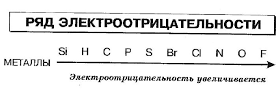
\includegraphics[width=0.7\linewidth]{21.electric}
	\caption{Ряд электроотрицательности (фрагмент)}
	\label{fig:21.electric}
\end{figure}


Галогены, азот, кислород, водород как простые вещества существуют в виде двухатомных молекул (\ce{F2, Cl2, Br2, I2, N2, O2, H2}). Остальные неметаллы могут существовать при нормальных условиях, как в кристаллическом состоянии, так и в аморфном состоянии. Неметаллы в отличие от металлов плохо проводят теплоту и электрический ток.

Для неметаллов также характерно проявление \textbf{аллотропии} --- существования элемента в форме различных простых веществ, различающихся либо строением и составом молекул (кислород и озон), либо способом упаковки (алмаз и графит). Пример аллотропных модификаций приведен на примере фосфора на рисунке \ref{fig:21.p}.

\begin{figure}[H]
	\centering
	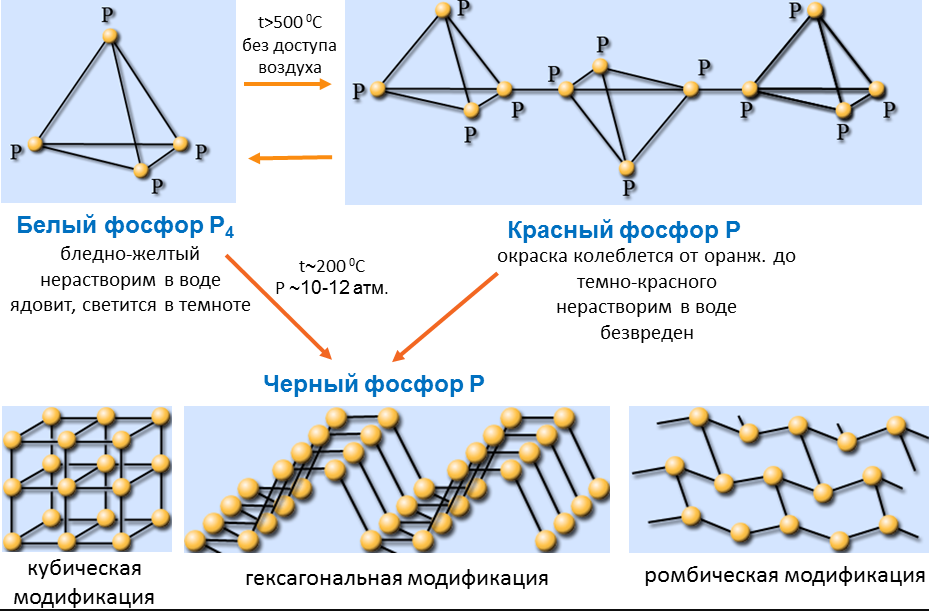
\includegraphics[width=0.7\linewidth]{21.p}
	\caption{Аллотропные модификации фосфора}
	\label{fig:21.p}
\end{figure}

\subsection{Химические свойства неметаллов}

Наиболее характерными степенями окисления для неметаллов являются отрицательные степени окисления, т.к/т.е. в большинстве реакций они выступают в роли окислителей. Иногда, при взаимодействии с более электроотрицательными неметаллами, например, они могут проявлять восстановительные свойства и принимать положительные степени окисления.

Если неметалл может образовывать соединения с разными степенями окисления, то свойства соединений будут зависеть от степени окисления элемента. С увеличением степени окисления кислотные свойства соединений увеличиваются.

\begin{enumerate}
	\item Для неметаллов характерны реакции с металлами, при это они проявляют окислительные свойства и в образующихся бинарных соединениях проявляют отрицательную степень окисления:
	
	\begin{align}
		\ce{Ca + H2 -> CaH2}\\
		\ce{2 Ca + O2 -> 2CaO}
 	\end{align}

	\item Неметаллы могут также взаимодействовать и с другими неметаллами, при этом более электроотрицательный металл играет роль окислителя, менее электроотрицательный --- роль восстановителя:
	
	\begin{align}
		\ce{S + 3 F2 -> SF6} \\
		\ce{H2 + Cl2 -> 2HCl}
	\end{align}

	При реакции с водородом неметаллы образуют летучие соединения (в обычных условиях это газы). Их водные растворы могут проявлять как основные (NH3, PH3), так и кислотные (\ce{HCl, HF}) свойства. В периоде с увеличением заряда ядра кислотные свойства водородных соединений неметаллов в водных растворах увеличиваются.

	При реакции с кислородом неметаллы образуют кислотные оксиды, проявляющие кислотные свойства. Они увеличиваются в периоде и уменьшаются в группе.

	При этому наиболее типичные неметаллы --- галогены (\ce{F}, \ce{Cl}, \ce{Br}, \ce{I}) --- с кислородом не реагируют (строго говоря, соединения попросту являются неустойчивыми), однако их можно получить косвенным путем, например \ce{F2O} можно получить при пропускании фтора через 2\%-ый водный раствор \ce{NaOH}:
	
	\begin{equation}
		\ce{2F2 + 2NaOH -> F2O + 2NaF + H2O}
	\end{equation}

	Однако, как и было сказано, подобная реакция очень капризна к условиям и при увеличении концентрации \ce{NaOH} выход \ce{F2O} резко уменьшится из-за протекания побочной реакции:
	
	\begin{equation}
		\ce{F2O + 2NaOH -> O2 + 2NaF + H2O}
	\end{equation}
\end{enumerate}